% Indicate the main file. Must go at the beginning of the file.
% !TEX root = ../main.tex

%%%%%%%%%%%%%%%%%%%%%%%%%%%%%%%%%%%%%%%%%%%%%%%%%%%%%%%%%%%%%%%%%%%%%%%%%%%%%%%%
% 04_discussion
%%%%%%%%%%%%%%%%%%%%%%%%%%%%%%%%%%%%%%%%%%%%%%%%%%%%%%%%%%%%%%%%%%%%%%%%%%%%%%%%


\section{Discussion}
\label{discussion}

\subsection{Detection}
- why \textit{mustela\_erminea} was so much more effected

- some examples for very nice BBoxes and some bad ones

Browsing trough the incorrectly predicted images with a high confidence value, it was found that many of the images contained a snail in the highest confidence BBox. A hand-picked selection of these images is shown in \autoref{fig:false_class_snails}.


\begin{figure}[]
\centering
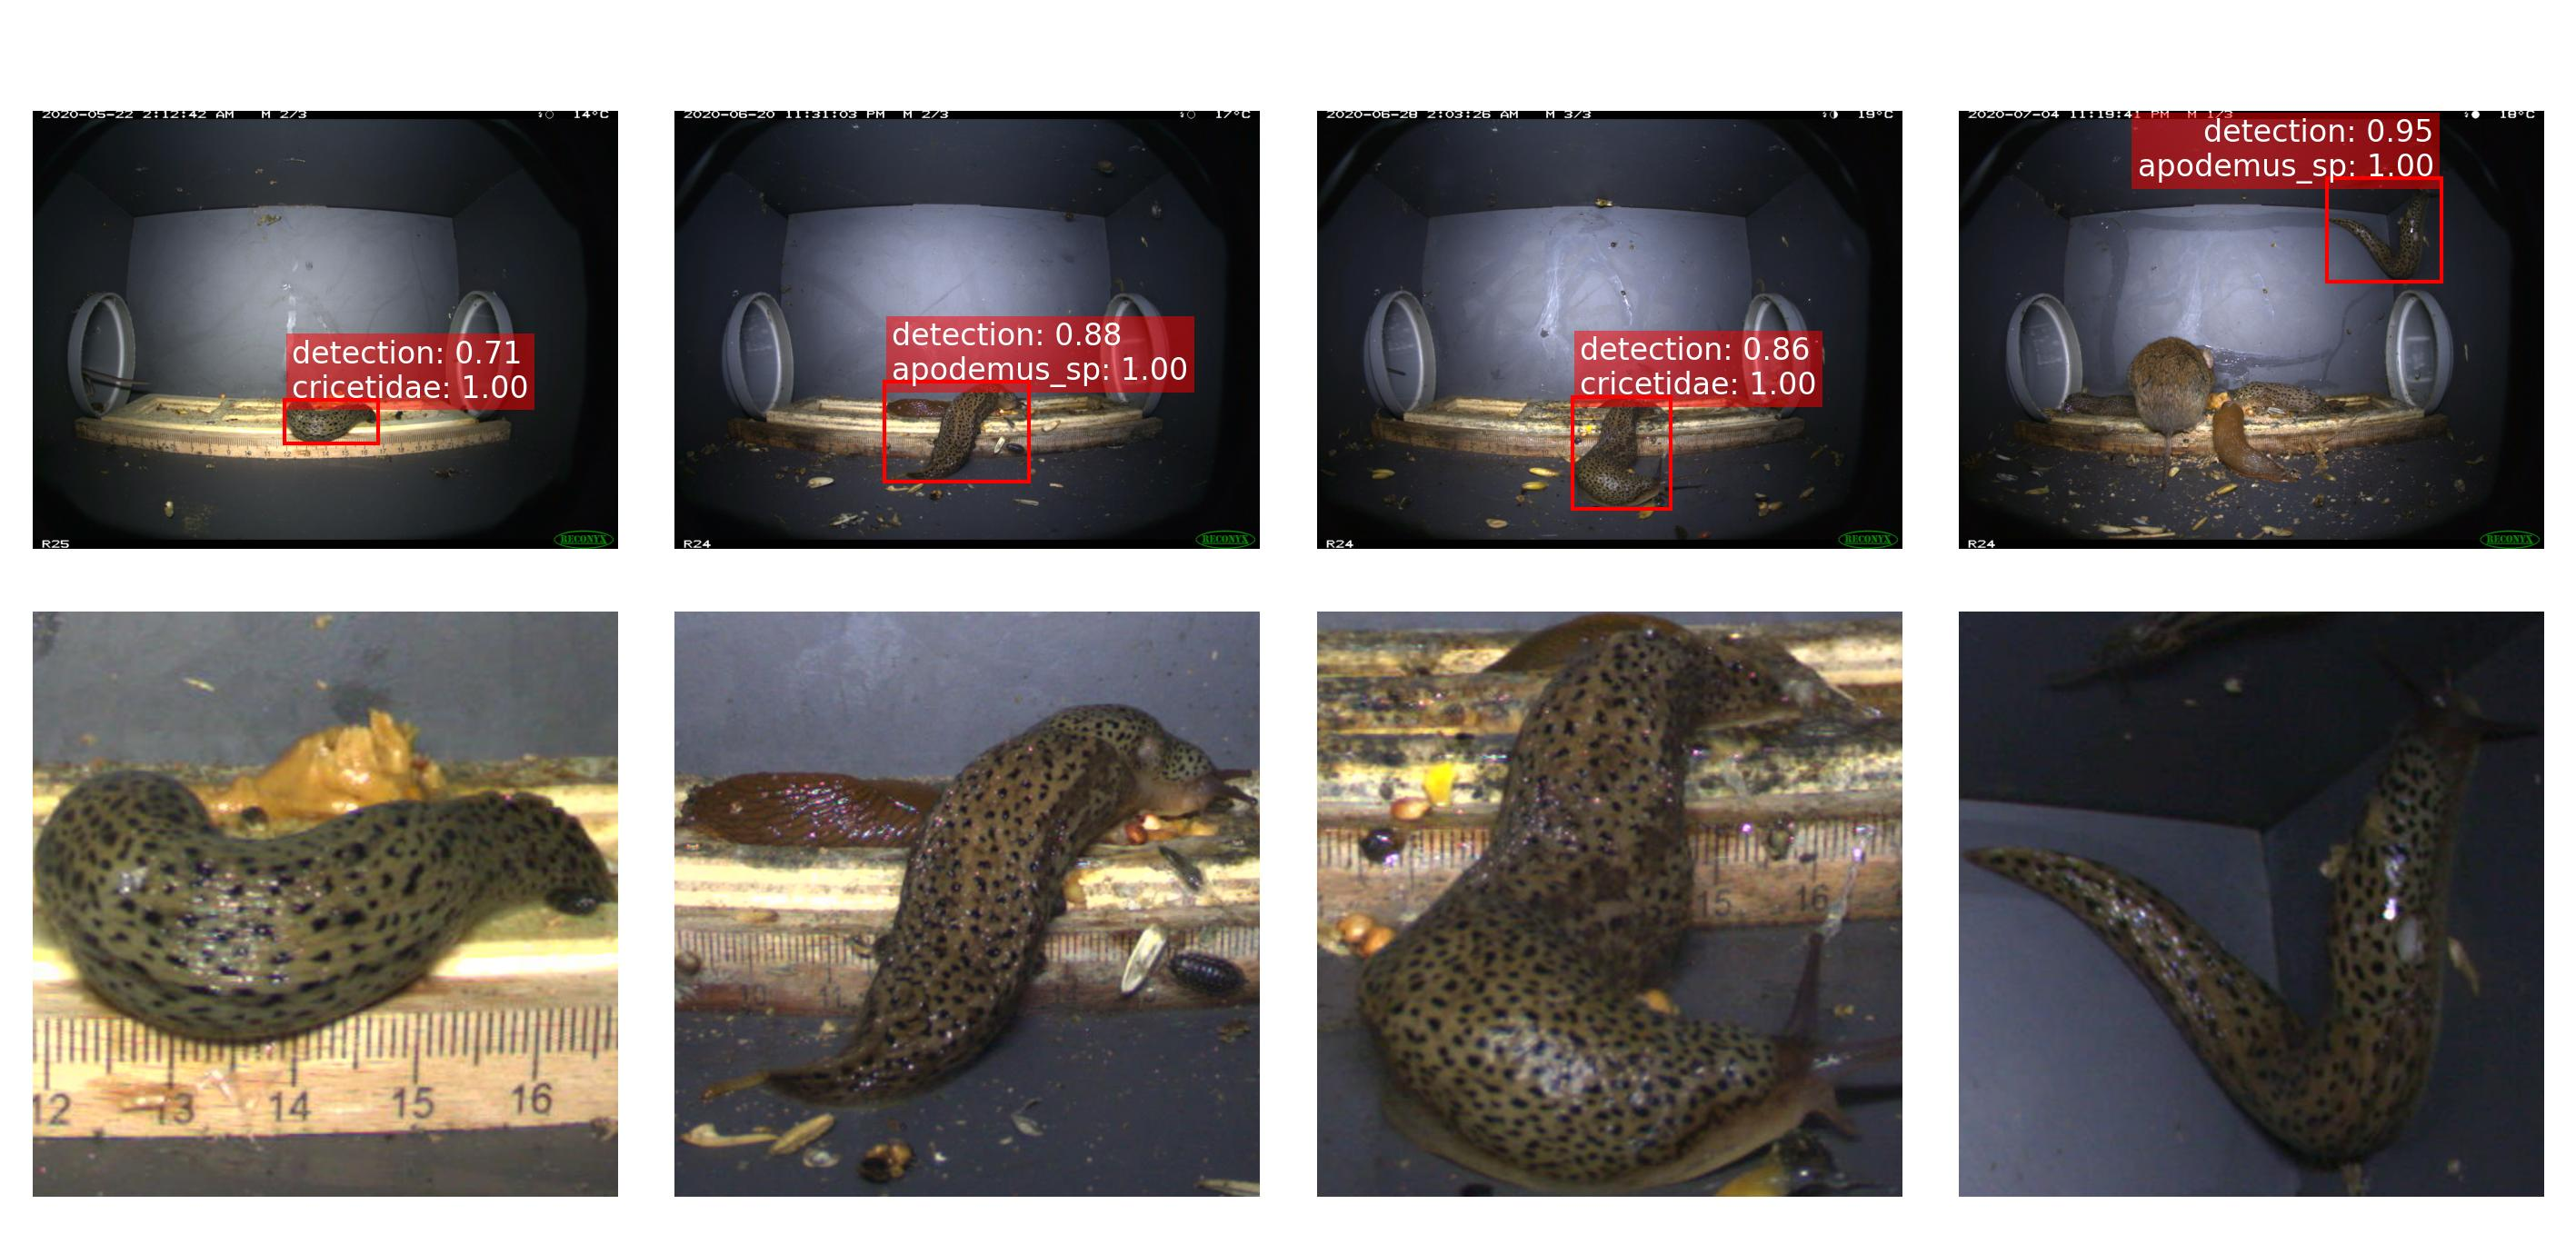
\includegraphics[width=\textwidth]{figures/false_class_snails.pdf}
\caption{Hand-picked selection of images predicted incorrectly with a high confidence value displaying a snail in the highest confidence BBox.}
\label{fig:false_class_snails}
\end{figure}

\subsection{Model Performance}
- discussing high model performance

- discuss benefit of pretrained models

- smaller vs larger models

\subsection{Best Model}

- discuss trainingmetrics and the fact it was trained so quickly

- do better detections mean better predictions?



\subsection{Limitations}

The biggest limitation of the currant approach is the lack of a extra class for samples that do not fall into any of the available categories forcing the model to make a decision even if this is not reasonable.
A very good example for this is the snail problem, where the model is forced to classify a snail as one of the available mammel categories as shown in \autoref{fig:false_class_snails}.

An other issue is the fact that the detector is still missing out on quite a few very promissing detections as demonstrated in \autoref{fig:detection_special_nodetect} or 


- this brute force approach is dependent on the amount of data available (rare species means less data)


new data generated info to discuss:
It is worth noting that in future use cases, the sequence length will likely be more standardized.
The actual length will depend on the camera settings -- common settings such as 1, 3, 5, or 10 images per trigger -- which can be extracted from the EXIF information of the images.

Data augmentation a well established way to improve model's generalization \autocite{shortenSurveyImageData2019} was implemented and considered as an option but not actually used in the end.